\section{Introduction}
\label{sec:intro}
% \begin{figure*}[t]
%     \centering
%     \begin{subfigure}{0.3\linewidth}
%         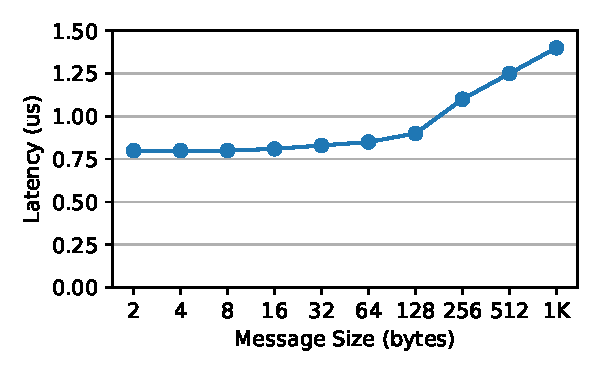
\includegraphics[width=0.99\linewidth]{fig/rdma_latency.pdf}
%         \label{fig:rdma_latency}
%         % \caption{}
%     \end{subfigure}.
%     \begin{subfigure}{0.3\linewidth}
%         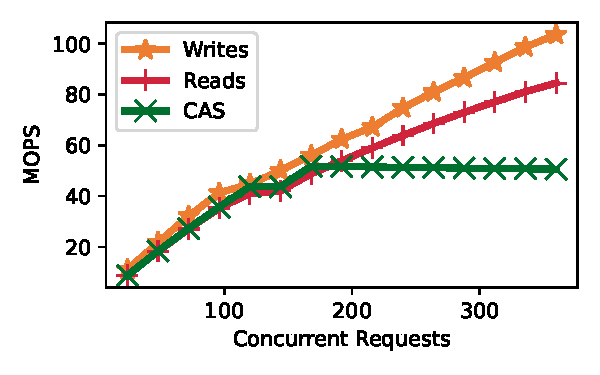
\includegraphics[width=0.99\linewidth]{fig/rdma_concur.pdf}
%         % \label{fig:optimistic_failures}
%         % \caption{}
%     \end{subfigure}
%     \begin{subfigure}{0.3\linewidth}
%         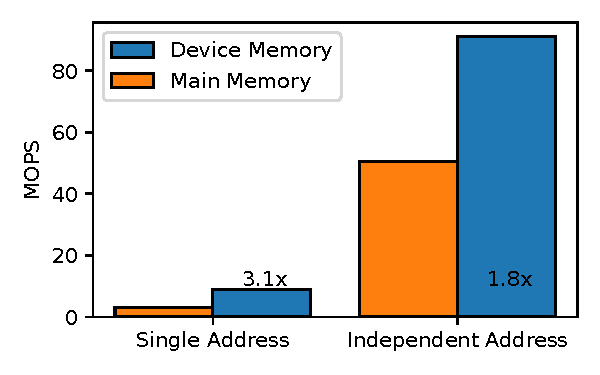
\includegraphics[width=0.99\linewidth]{fig/rdma_cas_throughput.pdf}
%         % \label{fig:optimistic_failures}
%         % \caption{}
%     \end{subfigure}
%     \vspace{-1em}
%     \caption{
%     \textbf{(a)} CX5 RDMA latency vs message size~\cite{rdma-latency}
%     \textbf{(b)} RDMA operation scalability
%     \textbf{(c)} Compare and swap performance. Device memory vs main memory.
%     }
%     \label{fig:rdma-benchmarks}
% \end{figure*}

% \begin{figure}[ht]
%     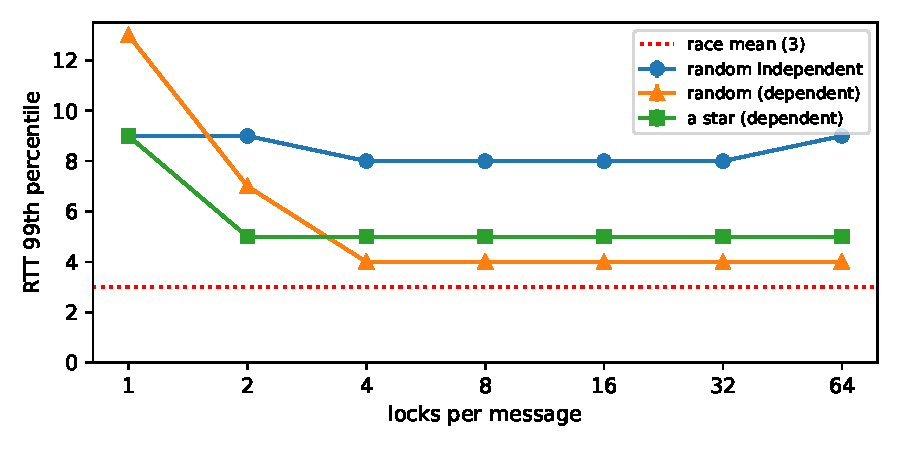
\includegraphics[width=0.99\linewidth]{fig/search_dependence.pdf}

%     \caption{Round trips per insert operation compared
%     across search functions and hash functions. Dependent
%     hash functions with A* have the shortest search
%     times.~\todo{latest numbers for A* are counter intuitive
%     - dig into}}

%     \label{fig:search_dependence}
% \end{figure}

\section{Rough Writing}

Black box disaggregation relies on an append only log
structure similar to black box numa. Clients commit
operations to the log by appending to the end of it. For
example inserting into a binary tree consists of first
appending the operation \textit{insert(value)} to the end of
the log. At this point in time the insert is serialized and
visible to all other clients. To read the inserted value the
client must read the entire log and then apply all of the
operations locally.

In order to perform a read the client runs a
\textit{read{value}} to the end of the log. After performing
the read the client can then apply all of the operations
locally and then perform the read.After performing the read
the client can then apply all of the operations locally and
then perform the read.

The hard issue with remote memory is getting seralization.
In the case of the the append only list a client must first
read to the end and then opportunistically append to the
end. Only at this point is the local operation valid. The
issue with this approach is two fold. Under high contention
the end of the log may continue to move resulting in a large
race condition between multiple clients, second the client
is never sure how much of the log to read in order to get to
the must up to date information. 

\textbf{append steering} This first problem can be solved
with a simple middlebox solution.  when operations are
appended to the end of the list a network middlebox caches
the tail of the list and steers the operation to the end of
the log. In this way, both insert, update, delete, and read
operations will achieve serialization in a single round
trip. 

\textbf{read infaltion} When clients need to read the log
they do not know how much of the log to read, as they cannot
determine how out of date they are. Again the middlebox can
inform the read. Giving an rdma read request to a known
location in the log a middlebox can inflate the read to the
end of the log enabling the client to capture all of the
operation in a single round trip. If a client is
significantly behind the middlebox can both maximize the
.ize of the read and inform the client of how much more must
be read. Take for instace a max read size of 5, with a
client that is 100 entries behind. The middlebox can inflate
the first read to size 5, and then report back to the client
that at least 19 more max sized reads are required. The
client can then batch those reads to reduce the time
required for the update to complete

\textbf{index structures}: Caching entire data structures
locally breaks the benefits of disaggregation, clients
should have small caches, however no caching leads to
extremely poor performance when dealing with contested
resources. We make the observation that in most cases index
structures are contested, while the stored data is usually
out of band from the index structures. As such we sugested
that node replication for disaggregation be used only on the
index structure. This enables clients to have all contention
removed, while storing only a small amount of data locally.

\textbf{high level algorithm} With no middle box the
algorithm for clients is simple. If they wish to perform an
operation they must first read to the end of the shared log
by performing iterative reads. After finding the end of the
log, they must issue a CAS operation which will append their
operation to the tail of the list. Once the operation is
appended the client serialization is complete on the index
structure. Depending on which operation was issued the
client can then complete the data path portion of the
operation. For reads the client must simply find the
location in the local index structer and then issue the
read. For writes the write must be commied prior to the data
being written to the index. For delete the value can simpley
be discarded and garbage collected later.

\textbf{optimized algorithm} With the middlebox the
operations are simpler. First for both read and write the
client can begin by issuing their data path operation
oportunistically, for the client the read can be sent out
ahead of all other requests, and for the write the data
portion can simply be written. Then the client issues a
write with a special header for the middlebox with the
contents of their appended operation in the message.
Alongside the append the client issues a read with a max
sized buffer allocated for the response. The middle box
ignores the opportunistic reads and datapath write. upon
seeing the append, the middlebox steers it to the end of the
list, and upon seeing the read of the log, it inflates the
read to the correct size. Including the operation which it
commited itself

Once the client receives the response it can determine its
next step. In the case of writes the operation will always
succed in a single round trip. In the case of reads the
client must first reconstruct its local index to determine
if it's opportunistic read is valid. If after reconstucting
the index teh clients read is valid it may contune on. If
the opprotnistic read was stale, the client must reissue a
read. This technique enables all writes to finish in a
single round trip, and all reads to finish in a max of 2
round trips depending on how stale their local cache is.


